\section{Conclusion: From Pythagoras to High-Frequency Trading (One Crisis at a Time)}

\subsection{How We Broke Math, Then Monetized It}

Somehow, we've gone from Pythagoras freaking out over irrational numbers to hedge funds running their own private arms race, executing trades faster than the SEC can blink. And, it wasn’t because mathematicians sat around sipping tea and contemplating the beauty of pure abstraction. No, it was because each era hit a mathematical crisis so baffling that we had no choice but to invent new math just to survive.

\begin{itemize}
    \item Galileo couldn't describe forces? We got calculus.
    \item Fourier broke math with infinite sums? We got real analysis.
    \item Cantor made infinity weird? We got set theory.
    \item Riemann integration couldn't handle chaotic functions? Enter Lebesgue.
    \item Big banks couldn't make money fast enough? We got high-frequency trading.
\end{itemize}

So, if you've made it this far, \textbf{congratulations, you’re now a quant.}

\begin{figure}[H]
\centering
\begin{tikzpicture}[every node/.style={font=\footnotesize}]

% Panel 1 — Pythagoras
\comicpanel{0}{4}
  {Pythagoras}
  {}
  {\textbf{Pythagoras:} What is the nature of number? Can the universe be measured?}
  {(0,-0.6)}

% Panel 2 — Newton
\comicpanel{6.5}{4}
  {Newton}
  {}
  {\textbf{Newton:} Does motion follow divine law, and can we measure its mechanics?}
  {(0,-0.6)}

% Panel 3 — Cantor
\comicpanel{0}{0}
  {Cantor}
  {}
  {\textbf{Cantor:} Is infinity a single concept, or a landscape of sizes and hierarchies?}
  {(0,0.8)}

% Panel 4 — Quant
\comicpanel{6.5}{0}
  {Quant}
  {}
  {\textbf{Quant:} If I embed Lebesgue measures in a trading model, can I short causality?}
  {(0,0.8)}

\end{tikzpicture}
\caption{Math broke, we fixed it then used it to outpace reality.}
\end{figure}



\subsection{Why the Smartest Mathematicians Work in Finance (and Not for You)}

The real secret of modern finance isn’t hidden in some dusty textbook or sealed away in a Swiss vault. It’s right there in the open — pulsing through server farms in New Jersey, whispered in nanoseconds between exchanges, dressed up like math but walking like a heist.

And I’ve just gone and spilled it.  So if I suddenly disappear after publishing this... you'll know why. 

\begin{quote}
High-frequency trading firms are not analysts, and they’re not investors. They’re financial hitmen with PhDs. They don’t play the market; they execute it. Arbitrage is their bullet, speed is their silencer, and you never see the trade until it’s already settled... and you’re already bleeding slippage.
\end{quote}

But really, explaining how this is like revealing that "tax efficiency" really means "financially engineering all your profits to go offshore," or that "integrating with investors" really means "lie to them, but make it legal."

That is, unless you’ve drunk the Kool-Aid: then "complex derivatives" are just innovative financial solutions, "structured products" are purely about risk management, and "market-making" has nothing to do with front-running clients.

\begin{figure}[H]
\centering
\figureseparator
\
\begin{minipage}{\linewidth}
\centering
\begin{tikzpicture}[node distance=5cm, every node/.style={align=center, font=\small}]
  % Market Maker node
  \node[draw, rounded corners, fill=blue!10, minimum width=4cm, minimum height=2cm] (maker) 
    {Market Maker\\ \textit{“Adds Liquidity”}};

  % Front-runner node (use relative positioning via node distance)
  \node[right=of maker, draw, rounded corners, fill=red!10, minimum width=4cm, minimum height=2cm] (runner)
    {Front Runner\\ \textit{“Acts Swiftly”}};

  % Centered Arrow with Label
  \draw[->, thick] (maker) -- node[above, midway] {\textbf{Receives Client Order}} (runner);

  % Dashed box implying identity
  \node[fit={(maker) (runner)}, draw=gray, dashed, thick, inner sep=0.4cm] (box) {};

  % Label just above the box
  \node[anchor=south] at ([yshift=4pt]box.north) 
    {\itshape \textbf{Just two completely unrelated roles... often performed on the same infrastructure.}};

  % Label just below the box
  \node[anchor=north, text width=11cm, align=center, font=\footnotesize] 
    at ([yshift=-4pt]box.south) 
    {Some people say this looks like front-running.\\\ \\ Others say it’s just efficient market participation.\\\ \\
    \textit{We say: it depends who's asking.}};
\end{tikzpicture}
\end{minipage}

\vspace{0.5em}
\caption{Market Making vs. Front Running: A Totally Innocent Overlap}
\caption*{\textit{These two things are obviously very different.\\ Don’t ask too many questions.}}
\figureseparator
\end{figure}


\vspace{1em}

And in case you think finance is just for MBAs and Wall Street bros, let me remind you: the industry that hires the most mathematicians and physicists isn’t academia: it’s finance. There's a reason why Wall Street poaches talent from theoretical physics and number theory faster than universities can replace them. Even Bill Gates once admitted that the company he feared the most wasn’t another tech giant: it was Goldman Sachs. 

And honestly? He had a point. Because at the end of the day, \textbf{mathematics has always been about power.}

So… what’s next? 

We’ve patched up the old gaps, cleaned up the messy edges, and wrapped everything in a rigorous framework. However, when math gets too comfortable, it gets boring. Maybe what we really need is another crisis: something so baffling, so frustrating, that it forces us to throw everything we know out the window and start fresh. 

Because if Thomas Kuhn taught us anything, it’s that desperation is the only true source of good ideas. And if history is any guide, the next great mathematical breakthrough won’t come from academia: it’ll come from some poor soul staring at their screen at 3 AM, realizing that everything they thought they knew is wrong. Again. 

And if that crisis happens to involve finance? Well, let’s just hope Goldman Sachs doesn’t get there first. 


\begin{figure}[H]
\centering

% === First row ===
\begin{subfigure}[t]{0.45\textwidth}
\centering
\begin{tikzpicture}
  \comicpanel{0}{0}
    {Grad Student}
    {}
    {I just proved a lemma that generalizes a corollary of a theorem that no one uses.}
    {(0,-0.6)}
\end{tikzpicture}
\caption*{Academia: Proving things no one reads.}
\end{subfigure}
\hfill
\begin{subfigure}[t]{0.45\textwidth}
\centering
\begin{tikzpicture}
  \comicpanel{0}{0}
    {Quant}
    {}
    {I used measure theory to front-run \$40M of trades. Before lunch.}
    {(0,-0.6)}
\end{tikzpicture}
\caption*{Finance: Theorems with immediate cash flow.}
\end{subfigure}

\vspace{1em}

% === Second row ===
\begin{subfigure}[t]{0.45\textwidth}
\centering
\begin{tikzpicture}
  \comicpanel{0}{0}
    {Professor}
    {}
    {Want to research pure math? Here's a stipend and a coffee machine.}
    {(0,0.8)}
\end{tikzpicture}
\caption*{The university incentive package.}
\end{subfigure}
\hfill
\begin{subfigure}[t]{0.45\textwidth}
\centering
\begin{tikzpicture}
  \comicpanel{0}{0}
    {Goldman Sachs}
    {}
    {Here's \$500k, and unlimited cocaine and hookers.}
    {(0,0.8)}
\end{tikzpicture}
\caption*{The Goldman Sachs incentive package.}
\end{subfigure}

\caption{Why the smartest mathematicians work in finance (and not for you).}
\end{figure}

